\documentclass[10pt]{beamer}
\usepackage[utf8]{inputenc}
\usepackage[francais]{babel}
\usepackage[T1]{fontenc}
\usepackage[export]{adjustbox}
\newcommand\Fontvi{\fontsize{8}{7.2}\selectfont}
\usepackage{tabularx}
\usepackage{minted}
\usemintedstyle{colorful}
\definecolor{mygray}{gray}{0.95}
\newenvironment{code}{\captionsetup{type=listing}}{}

\usepackage{hyperref}
% \hypersetup{
%     colorlinks,
%     citecolor=black,
%     filecolor=black,
%     linkcolor=black,
%     urlcolor=blue
% }
\usepackage{graphicx}
\usepackage{multimedia}

\usetheme{Frankfurt}
\usecolortheme{default}

\addtobeamertemplate{navigation symbols}{}{%
    \usebeamerfont{footline}%
    \usebeamercolor[fg]{footline}%
    \hspace{1em}%
    \insertframenumber/\inserttotalframenumber
}

\titlegraphic{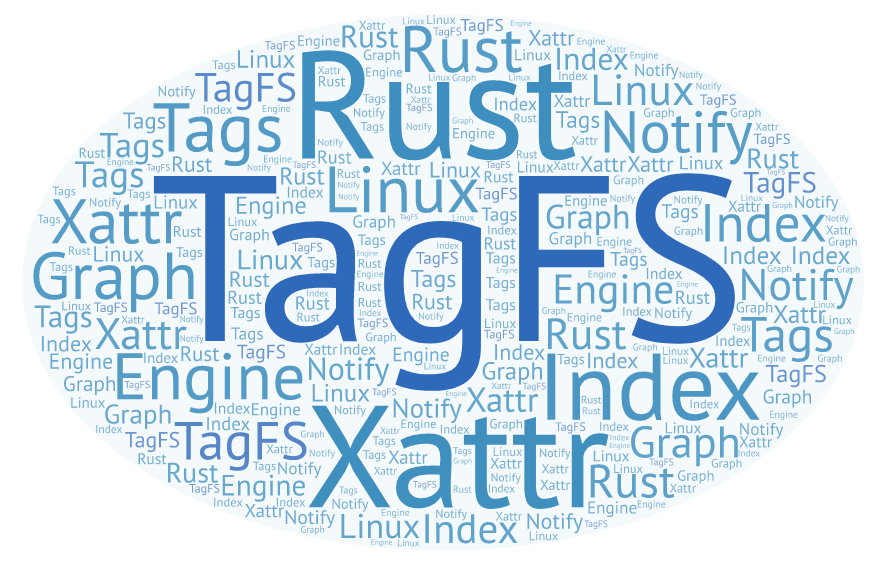
\includegraphics[width=0.5\textwidth]{images/title.png}}

\begin{document}
\logo{%
    \makebox[0.95\paperwidth]{%
        
\includegraphics[width=2.5cm,keepaspectratio]{images/hepia.jpg}%
        \hfill%
        
\includegraphics[width=2.5cm,keepaspectratio]{images/hesso.jpg}%
    }%
}

\title{TagFS - Système d'étiquetage des fichiers avec Rust}
\author{Steven Liatti}
\institute{Projet de bachelor - Prof. Florent Glück - Hepia ITI 3\up{ème} année}
\date{4 septembre 2018}

\begin{frame}
\titlepage
\end{frame}

\begin{frame}
    \frametitle{Plan}
    \setcounter{tocdepth}{1}
    \tableofcontents
\end{frame}

%%%%%%%%%%%%%%%%%%%%%%%%%%%%%%%%%%%%%%%%%%%%%%%%%%%%%%%%%%%%%%%%%%%%%%%%%%%%%%%%%%%%%%%%%%%%%%%%%%%
%%%%%%%%%%%%%%%%%%%%%%%%%%%%%%%%%%%%%%%%%%%%%%%%%%%%%%%%%%%%%%%%%%%%%%%%%%%%%%%%%%%%%%%%%%%%%%%%%%%
\section{Introduction}
\subsection{Problématiques}
\begin{frame}
    \frametitle{\subsecname}
    \begin{itemize}
        \item Nombre de fichiers énorme.
        \pause
        \item Difficulté à retrouver des fichiers.
        \pause
        \item Plusieurs emplacements logiques pour un seul fichier.
        \pause
    \end{itemize}
    \Large\textbf{Système de "tagging" de fichiers et répertoires avec possibilité de recherche par tags.}
\end{frame}

\subsection{Cahier des charges}
\begin{frame}
    \frametitle{\subsecname}
    \begin{itemize}
        \item Répertorier les applications existantes permettant d'étiqueter les fichiers.
        \pause
        \item Étudier les attributs étendus (XATTR) lors des manipulation courantes sur les fichiers.
        \pause
        \item Analyser les moyens d'indexer et de surveiller une arborescence de fichiers.
        \pause
        \item Concevoir et implémenter le système (open source et sur Linux) et mesurer ses performances.
        \pause
        \item Étudier et s'approprier le langage Rust.
    \end{itemize}
\end{frame}

%%%%%%%%%%%%%%%%%%%%%%%%%%%%%%%%%%%%%%%%%%%%%%%%%%%%%%%%%%%%%%%%%%%%%%%%%%%%%%%%%%%%%%%%%%%%%%%%%%%
%%%%%%%%%%%%%%%%%%%%%%%%%%%%%%%%%%%%%%%%%%%%%%%%%%%%%%%%%%%%%%%%%%%%%%%%%%%%%%%%%%%%%%%%%%%%%%%%%%%
\section{Solutions existantes}
\subsection{TMSU, Tagsistant et TagSpaces}
\begin{frame}
    \frametitle{\subsecname}
    \begin{columns}[T]
        \begin{column}{.35\textwidth}
        \fontsize{8pt}{9}\selectfont
            \begin{center}
                \begin{itemize}
                    \item Gestion des tags.
                    \item Liste de fichiers liés aux tags.
                    \item CLI ou GUI.
                \end{itemize}
                \pause[3]
                \bigbreak
                \begin{tabularx}{4.5cm}{|p{1.8cm}|X|} \hline
                    \textbf{Points positifs} & \textbf{Points négatifs} \\ \hline
                    Simples & Dépendance à une BDD externe \\ \hline
                    Rapides et efficaces & Modification et accès uniquement par l'app \\ \hline
                    Open source & \\ \hline
                \end{tabularx}
            \end{center}
        \end{column}
        \pause[2]
        \begin{column}{.65\textwidth}
            \begin{flushright}
                \begin{figure}
                    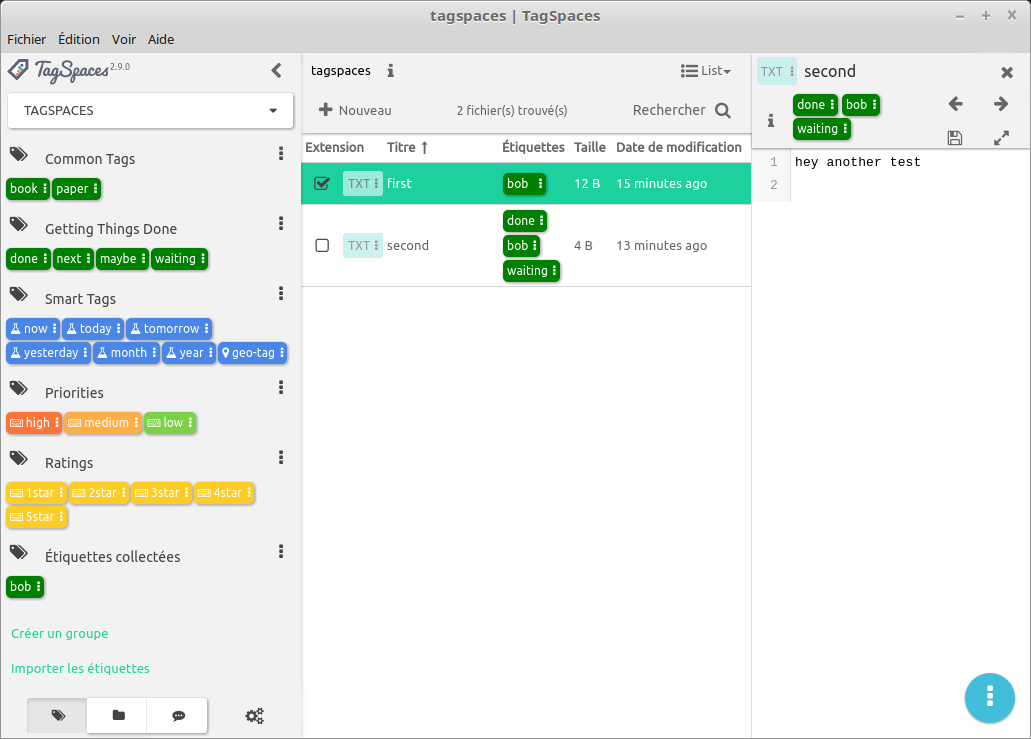
\includegraphics[width=0.98\textwidth]{images/tagspaces.png}
                \end{figure}
            \end{flushright}
        \end{column}
    \end{columns}
\end{frame}

\subsection{macOS}
\begin{frame}
    \frametitle{\subsecname}
    \fontsize{8pt}{9}\selectfont
    \begin{columns}[T]
        \begin{column}{.55\textwidth}
            \begin{center}
                \begin{figure}
                    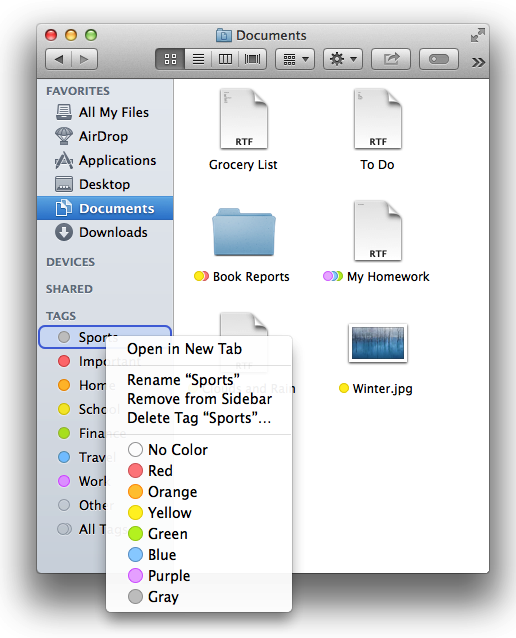
\includegraphics[width=0.7\textwidth]{images/macos_tags.png}
                    \caption{Gestion d'un tag dans le Finder \cite{ref5}}
                \end{figure}
            \end{center}
        \end{column}
        \pause
        \begin{column}{.45\textwidth}
            \begin{center}
                \begin{tabularx}{5.3cm}{|X|X|} \hline
                    \textbf{Points positifs} & \textbf{Points négatifs} \\ \hline
                    Système de tags intégré à l'explorateur de fichiers & Code propriétaire \\ \hline
                    Stocke les tags dans les XATTR & Seulement pour macOS \\ \hline
                    Performant & \\ \hline
                \end{tabularx}
            \end{center}
        \end{column}
    \end{columns}
\end{frame}

%%%%%%%%%%%%%%%%%%%%%%%%%%%%%%%%%%%%%%%%%%%%%%%%%%%%%%%%%%%%%%%%%%%%%%%%%%%%%%%%%%%%%%%%%%%%%%%%%%
%%%%%%%%%%%%%%%%%%%%%%%%%%%%%%%%%%%%%%%%%%%%%%%%%%%%%%%%%%%%%%%%%%%%%%%%%%%%%%%%%%%%%%%%%%%%%%%%%%
\section{Architecture}
\subsection{Gestion des tags}
\begin{frame}
    \frametitle{\subsecname}
    \begin{itemize}
        \item Stockage des tags dans les attributs étendus (XATTR).
        \pause
        \item Outil dédié plutôt que reprendre les commandes existantes \\ => Confort d'utilisation.
    \end{itemize}
\end{frame}

\subsection{Indexation des fichiers et des tags}
\begin{frame}
    \frametitle{\subsecname}
    \begin{columns}[T]
        \begin{column}{.6\textwidth}
            \begin{figure}
                \begin{center}
                    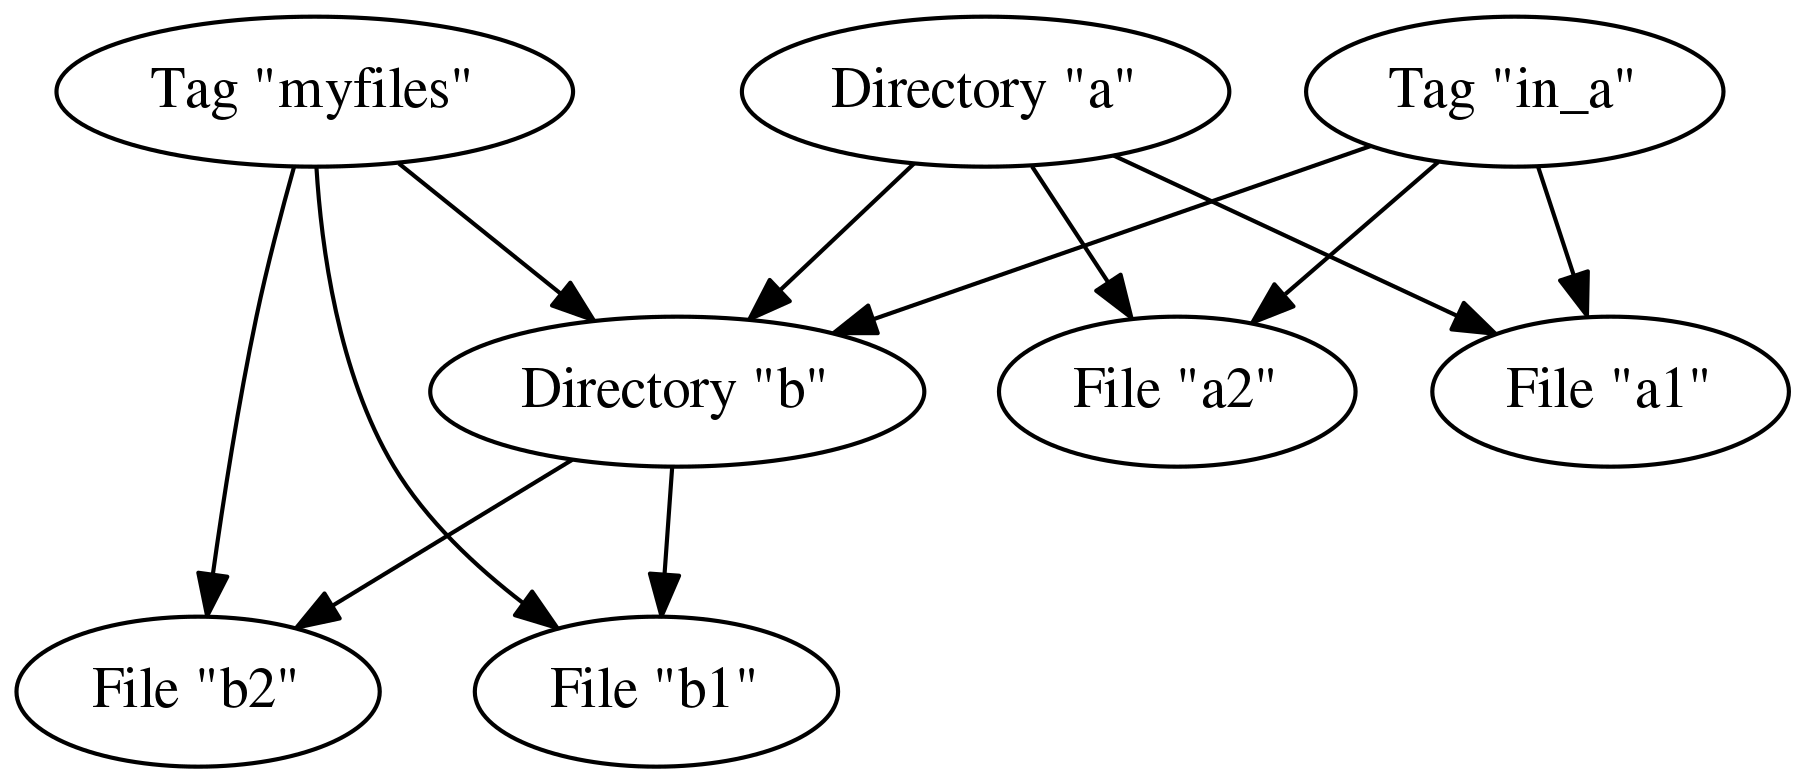
\includegraphics[width=1\textwidth]{images/graph.png}
                \end{center}
            \end{figure}
        \end{column}
        \pause
        \begin{column}{.4\textwidth}
            \begin{figure}
                \begin{center}
                    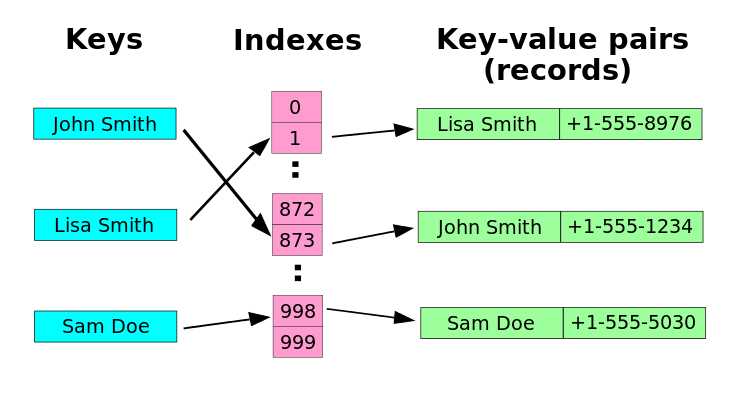
\includegraphics[width=1\textwidth]{images/hashmap_wiki.png}
                    \caption{Un annuaire représenté comme une table de hachage - \cite{ref27}}
                \end{center}
            \end{figure}
        \end{column}
    \end{columns}
\end{frame}

\subsection{Surveillance du système de fichiers}
\begin{frame}
    \frametitle{\subsecname}
    Mise à jour du graphe lors des événements suivants :
    \bigbreak
    \pause
    \begin{itemize}
        \item Changement sur les tags.
        \pause
        \item Création de fichiers/répertoires.
        \pause
        \item Suppression de fichiers/répertoires.
        \pause
        \item Déplacement/renommage de fichiers/répertoires.
    \end{itemize}
\end{frame}

\subsection{Requêtes de tags et fichiers}
\begin{frame}
    \frametitle{\subsecname}
    \begin{itemize}
        \pause
        \item Lister les fichiers et répertoires associés à des tags => requêtes sous forme 
            d'expressions logiques.
        \pause
        \item Lister les tags existants.
        \pause
        \item Renommer un tag.
    \end{itemize}
\end{frame}

%%%%%%%%%%%%%%%%%%%%%%%%%%%%%%%%%%%%%%%%%%%%%%%%%%%%%%%%%%%%%%%%%%%%%%%%%%%%%%%%%%%%%%%%%%%%%%%%%%%
%%%%%%%%%%%%%%%%%%%%%%%%%%%%%%%%%%%%%%%%%%%%%%%%%%%%%%%%%%%%%%%%%%%%%%%%%%%%%%%%%%%%%%%%%%%%%%%%%%%
\section{Technologies}
\subsection{Rust}
\subsubsection{Généralités}
\begin{frame}
    \frametitle{\subsecname}
    \framesubtitle{\subsubsecname}
    \begin{itemize}
        \item Langage système moderne, performant, fiable (plus sécurisé qu'Ada), compilé, et fortement typé.
        \pause
        \item Disponible sur Linux, Windows et macOS.
        \pause
        \item Cargo : outil de compilation et d'exécution et gestionnaire de paquets intégré à Rust.
        \pause
        \item Structures, collections, généricité, immutabilité, énumérations et \textit{pattern matching}.
        \pause
        \item Gestion des erreurs.
        \pause
        \item Tests.
    \end{itemize}
\end{frame}

\subsubsection{Ownership, Borrowing}
\begin{frame}
    \frametitle{\subsecname}
    \framesubtitle{\subsubsecname}
    \textbf{Ownership}
    \begin{itemize}
        \pause
        \item Chaque variable est dite le "possesseur" (\textit{owner}) d'une valeur.
        \pause
        \item Il ne peut y avoir qu'un seul \textit{owner} pour une valeur.
        \pause
        \item Lorsque l'\textit{owner} est détruit ou change de portée, la valeur est détruite.
    \end{itemize}
    \bigbreak
    \pause
    \textbf{Borrowing}
    \begin{itemize}
        \pause
        \item À tout moment, il ne peut exister qu'une seule référence mutable ou plusieurs 
            références immutables, mais pas les deux en même temps.
        \pause
        \item Les références doivent toujours être valides.
    \end{itemize}
\end{frame}

\subsection{Attributs étendus (XATTR)}
\begin{frame}
    \frametitle{\subsecname}
    \begin{itemize}
        \item Métadonnée sous forme de paire \mintinline{text}{nom:valeur}.
        \pause
        \item Nom = chaine de caractères, valeur = chaine de caractères ou données binaires.
        \pause
        \item Existent sous ext2-3-4, XFS, Btrfs, UFS1-2, NTFS, HFS+, ZFS.
        \pause
        \item Outils CLI pour facilement les manipuler.
    \end{itemize}
\end{frame}

\subsection{Inotify}
\begin{frame}
    \frametitle{\subsecname}
    \begin{itemize}
        \item API de notifications d'événements sur le système de fichiers.
        \pause
        \item Trois appels système : initialisation, ajout de surveillance sur un chemin de fichiers 
            donné et suppression de cette surveillance.
        \pause
        \item Lecture d'un événement avec read().
    \end{itemize}
\end{frame}

\subsection{Sockets}
\begin{frame}
    \frametitle{\subsecname}
    \begin{figure}
        \begin{center}
            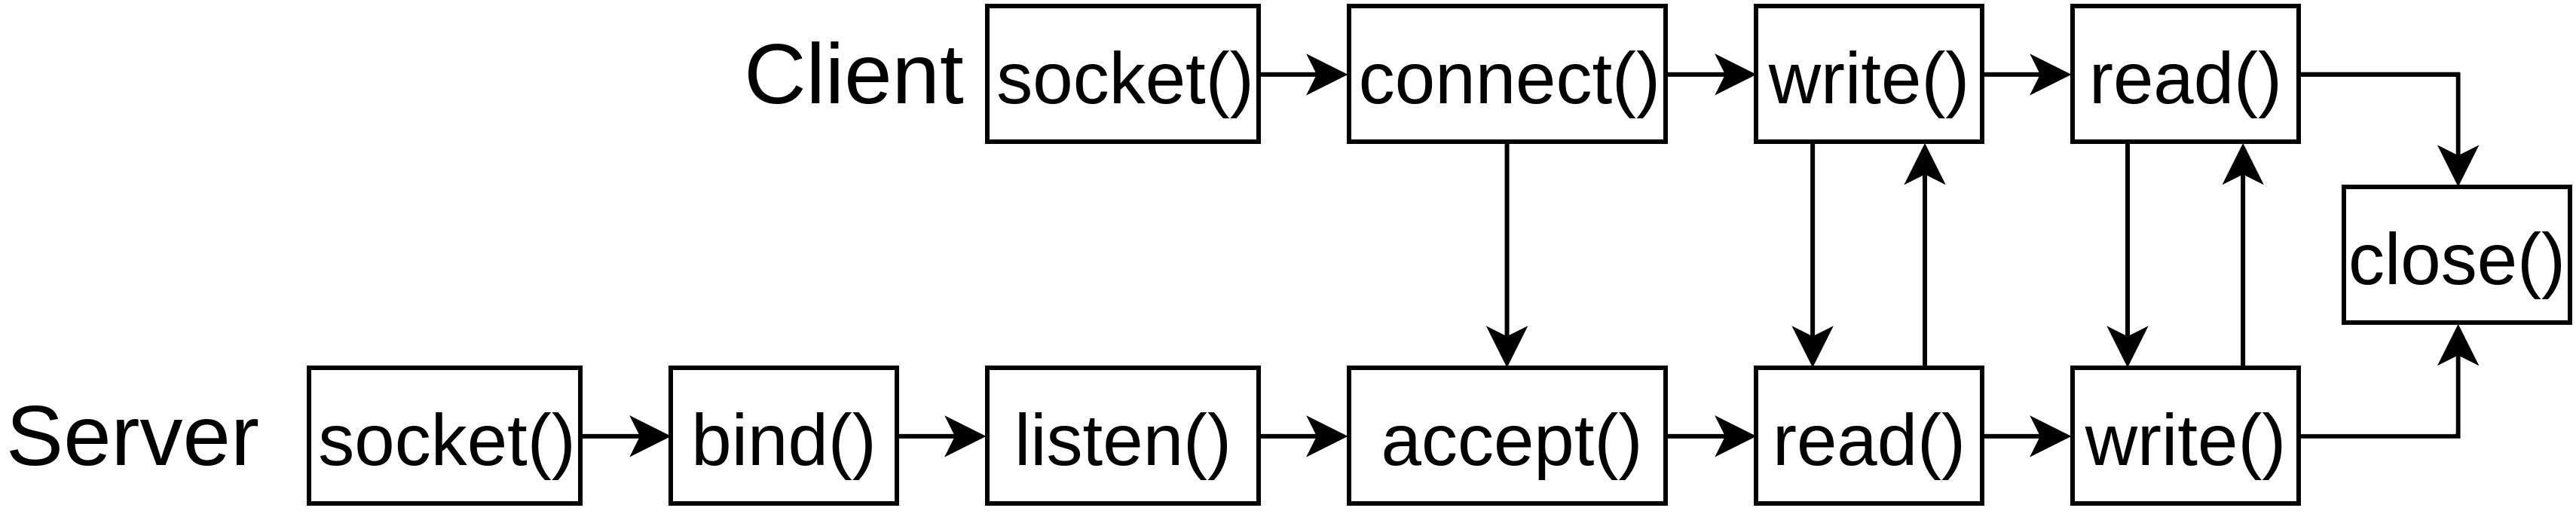
\includegraphics[width=1\textwidth]{images/sockets2.png}
        \end{center}
    \end{figure}
\end{frame}

%%%%%%%%%%%%%%%%%%%%%%%%%%%%%%%%%%%%%%%%%%%%%%%%%%%%%%%%%%%%%%%%%%%%%%%%%%%%%%%%%%%%%%%%%%%%%%%%%%%
%%%%%%%%%%%%%%%%%%%%%%%%%%%%%%%%%%%%%%%%%%%%%%%%%%%%%%%%%%%%%%%%%%%%%%%%%%%%%%%%%%%%%%%%%%%%%%%%%%%
\section{Réalisation}
\subsection{Tag Manager}
\begin{frame}
    \frametitle{\subsecname}
    \begin{columns}[T]
        \begin{column}{.5\textwidth}
            \begin{figure}
                \begin{center}
                    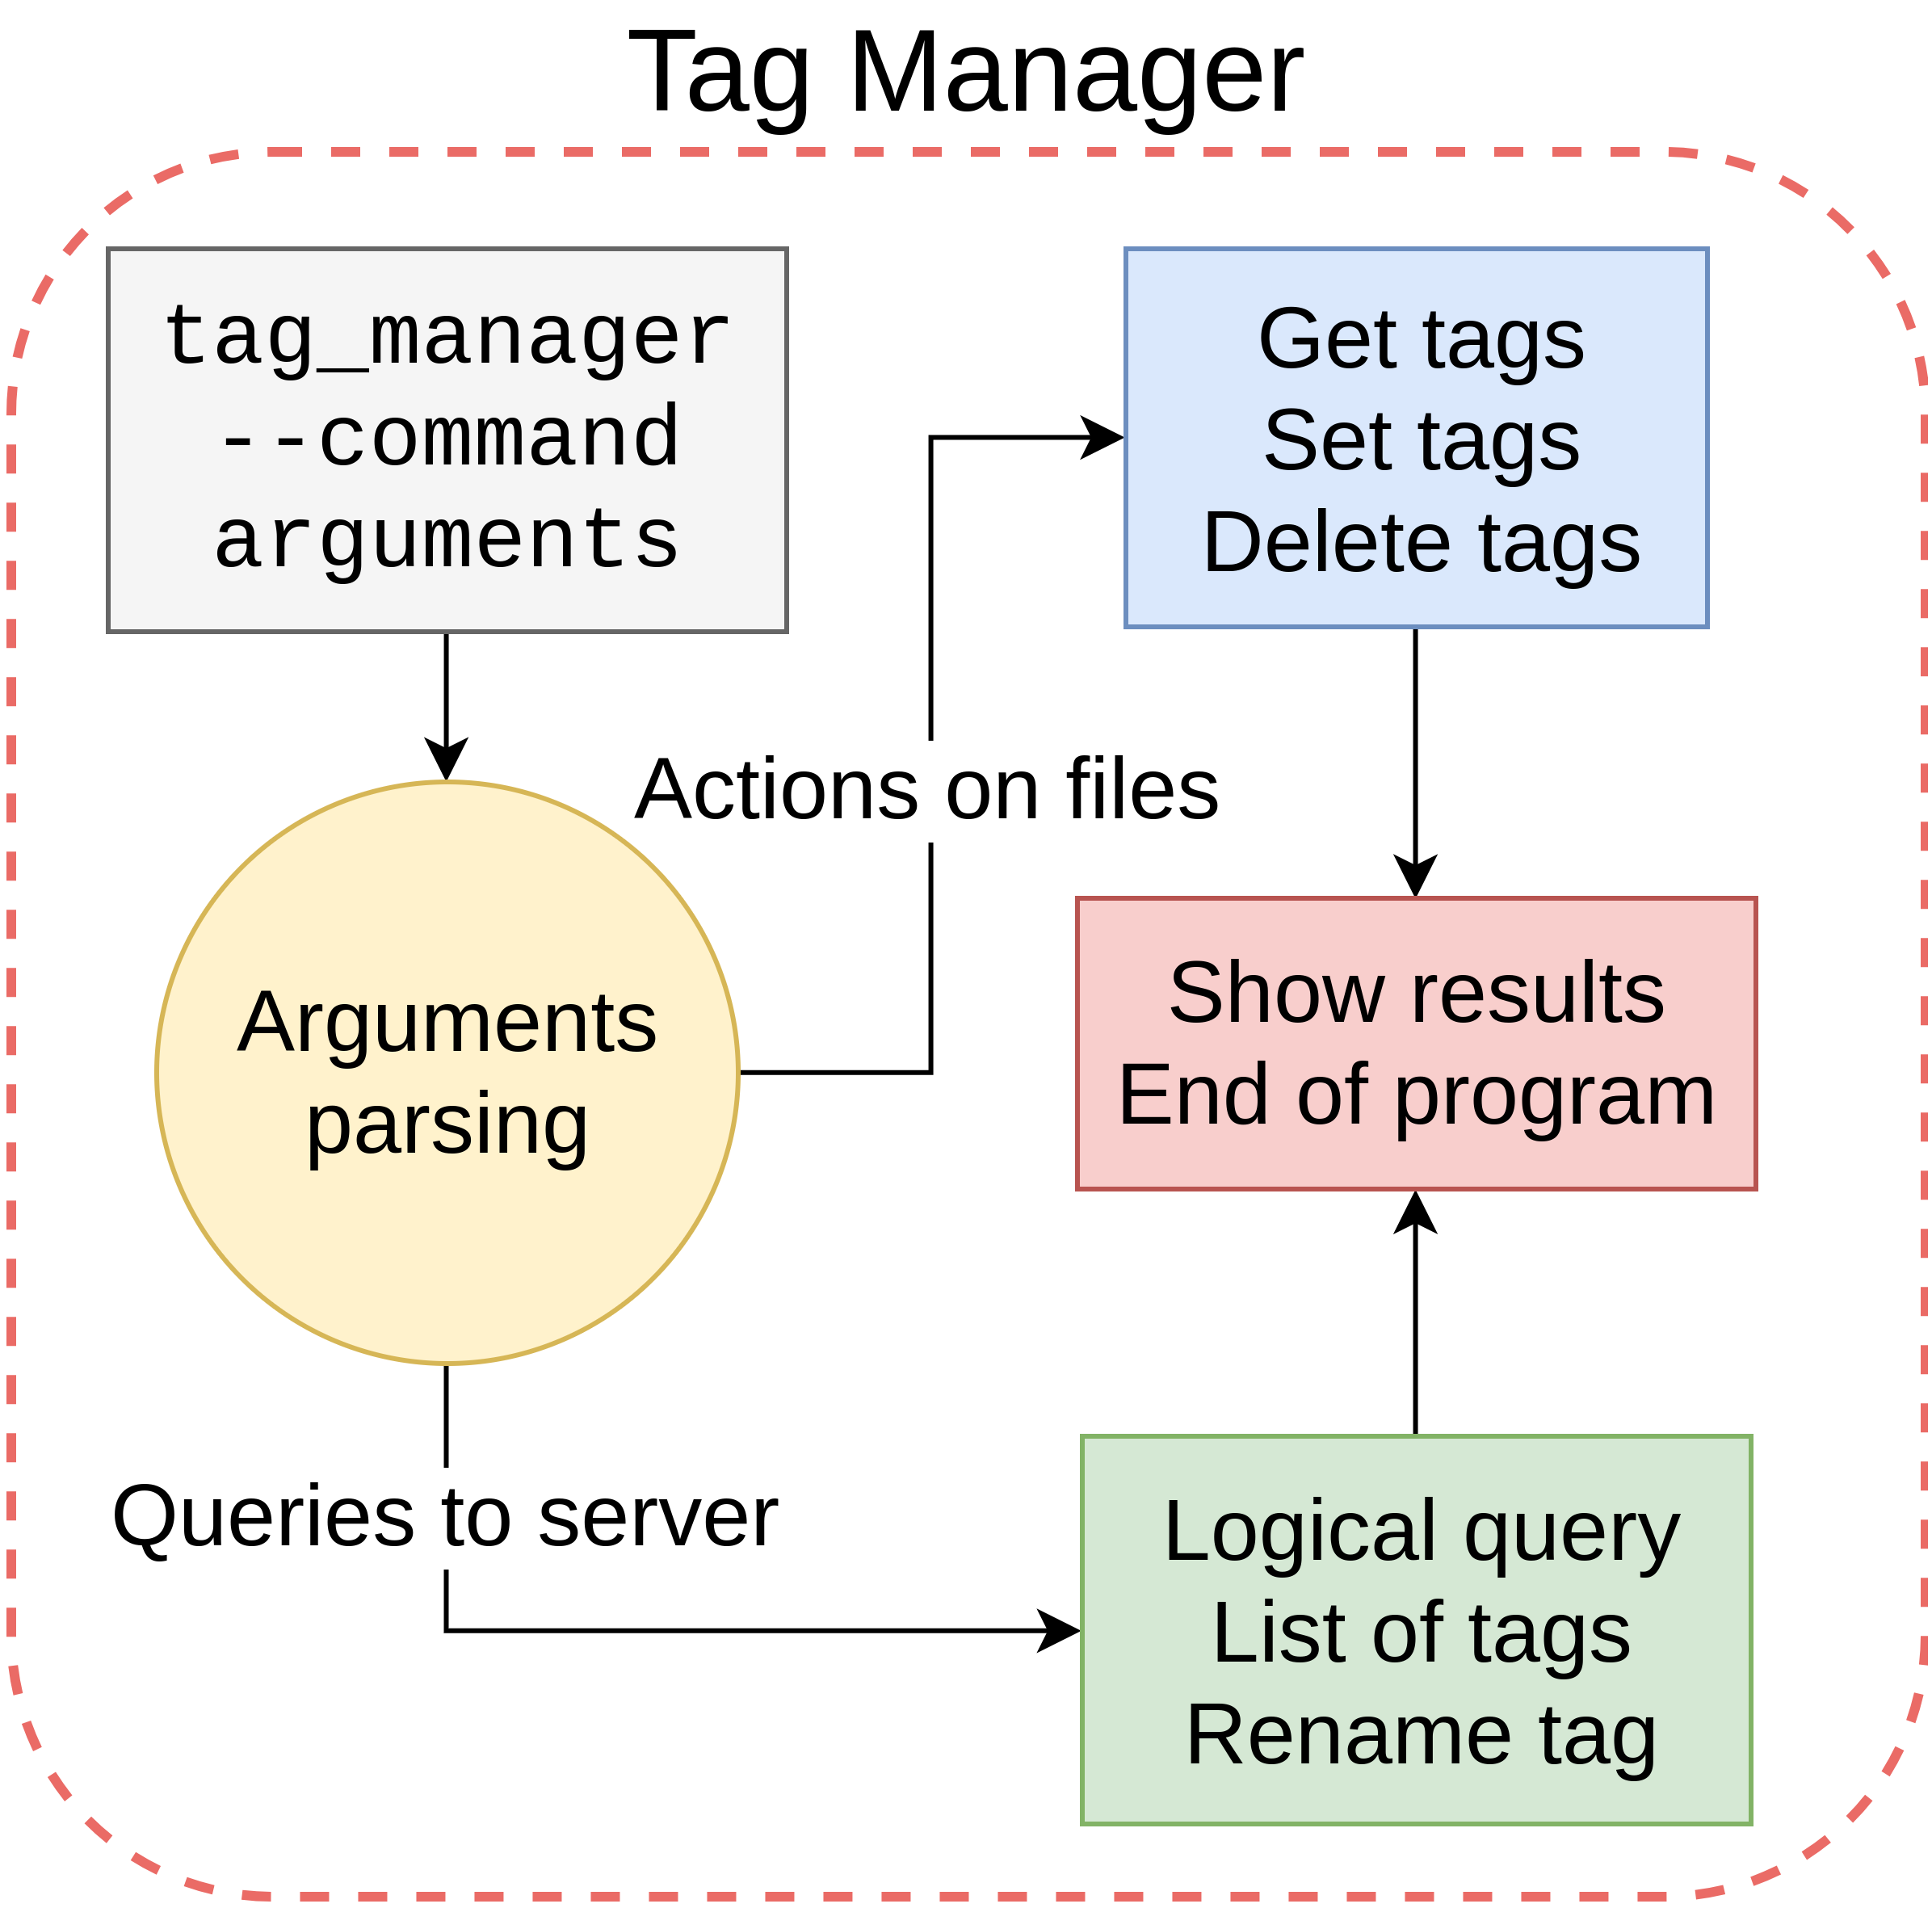
\includegraphics[width=1\textwidth]{images/tag_manager2.png}
                \end{center}
            \end{figure}
        \end{column}
        \pause
        \begin{column}{.5\textwidth}
            \begin{itemize}
                \item Programme "client".
                \item CLI.
                \item Gestion des tags.
                \item Manipule les XATTR des fichiers.
                \item Envoi de requêtes à Tag Engine.
            \end{itemize}
        \end{column}
    \end{columns}
\end{frame}

\subsection{Tag Engine}
\begin{frame}
    \frametitle{\subsecname}
    \begin{columns}[T]
        \begin{column}{.6\textwidth}
            \begin{figure}
                \begin{center}
                    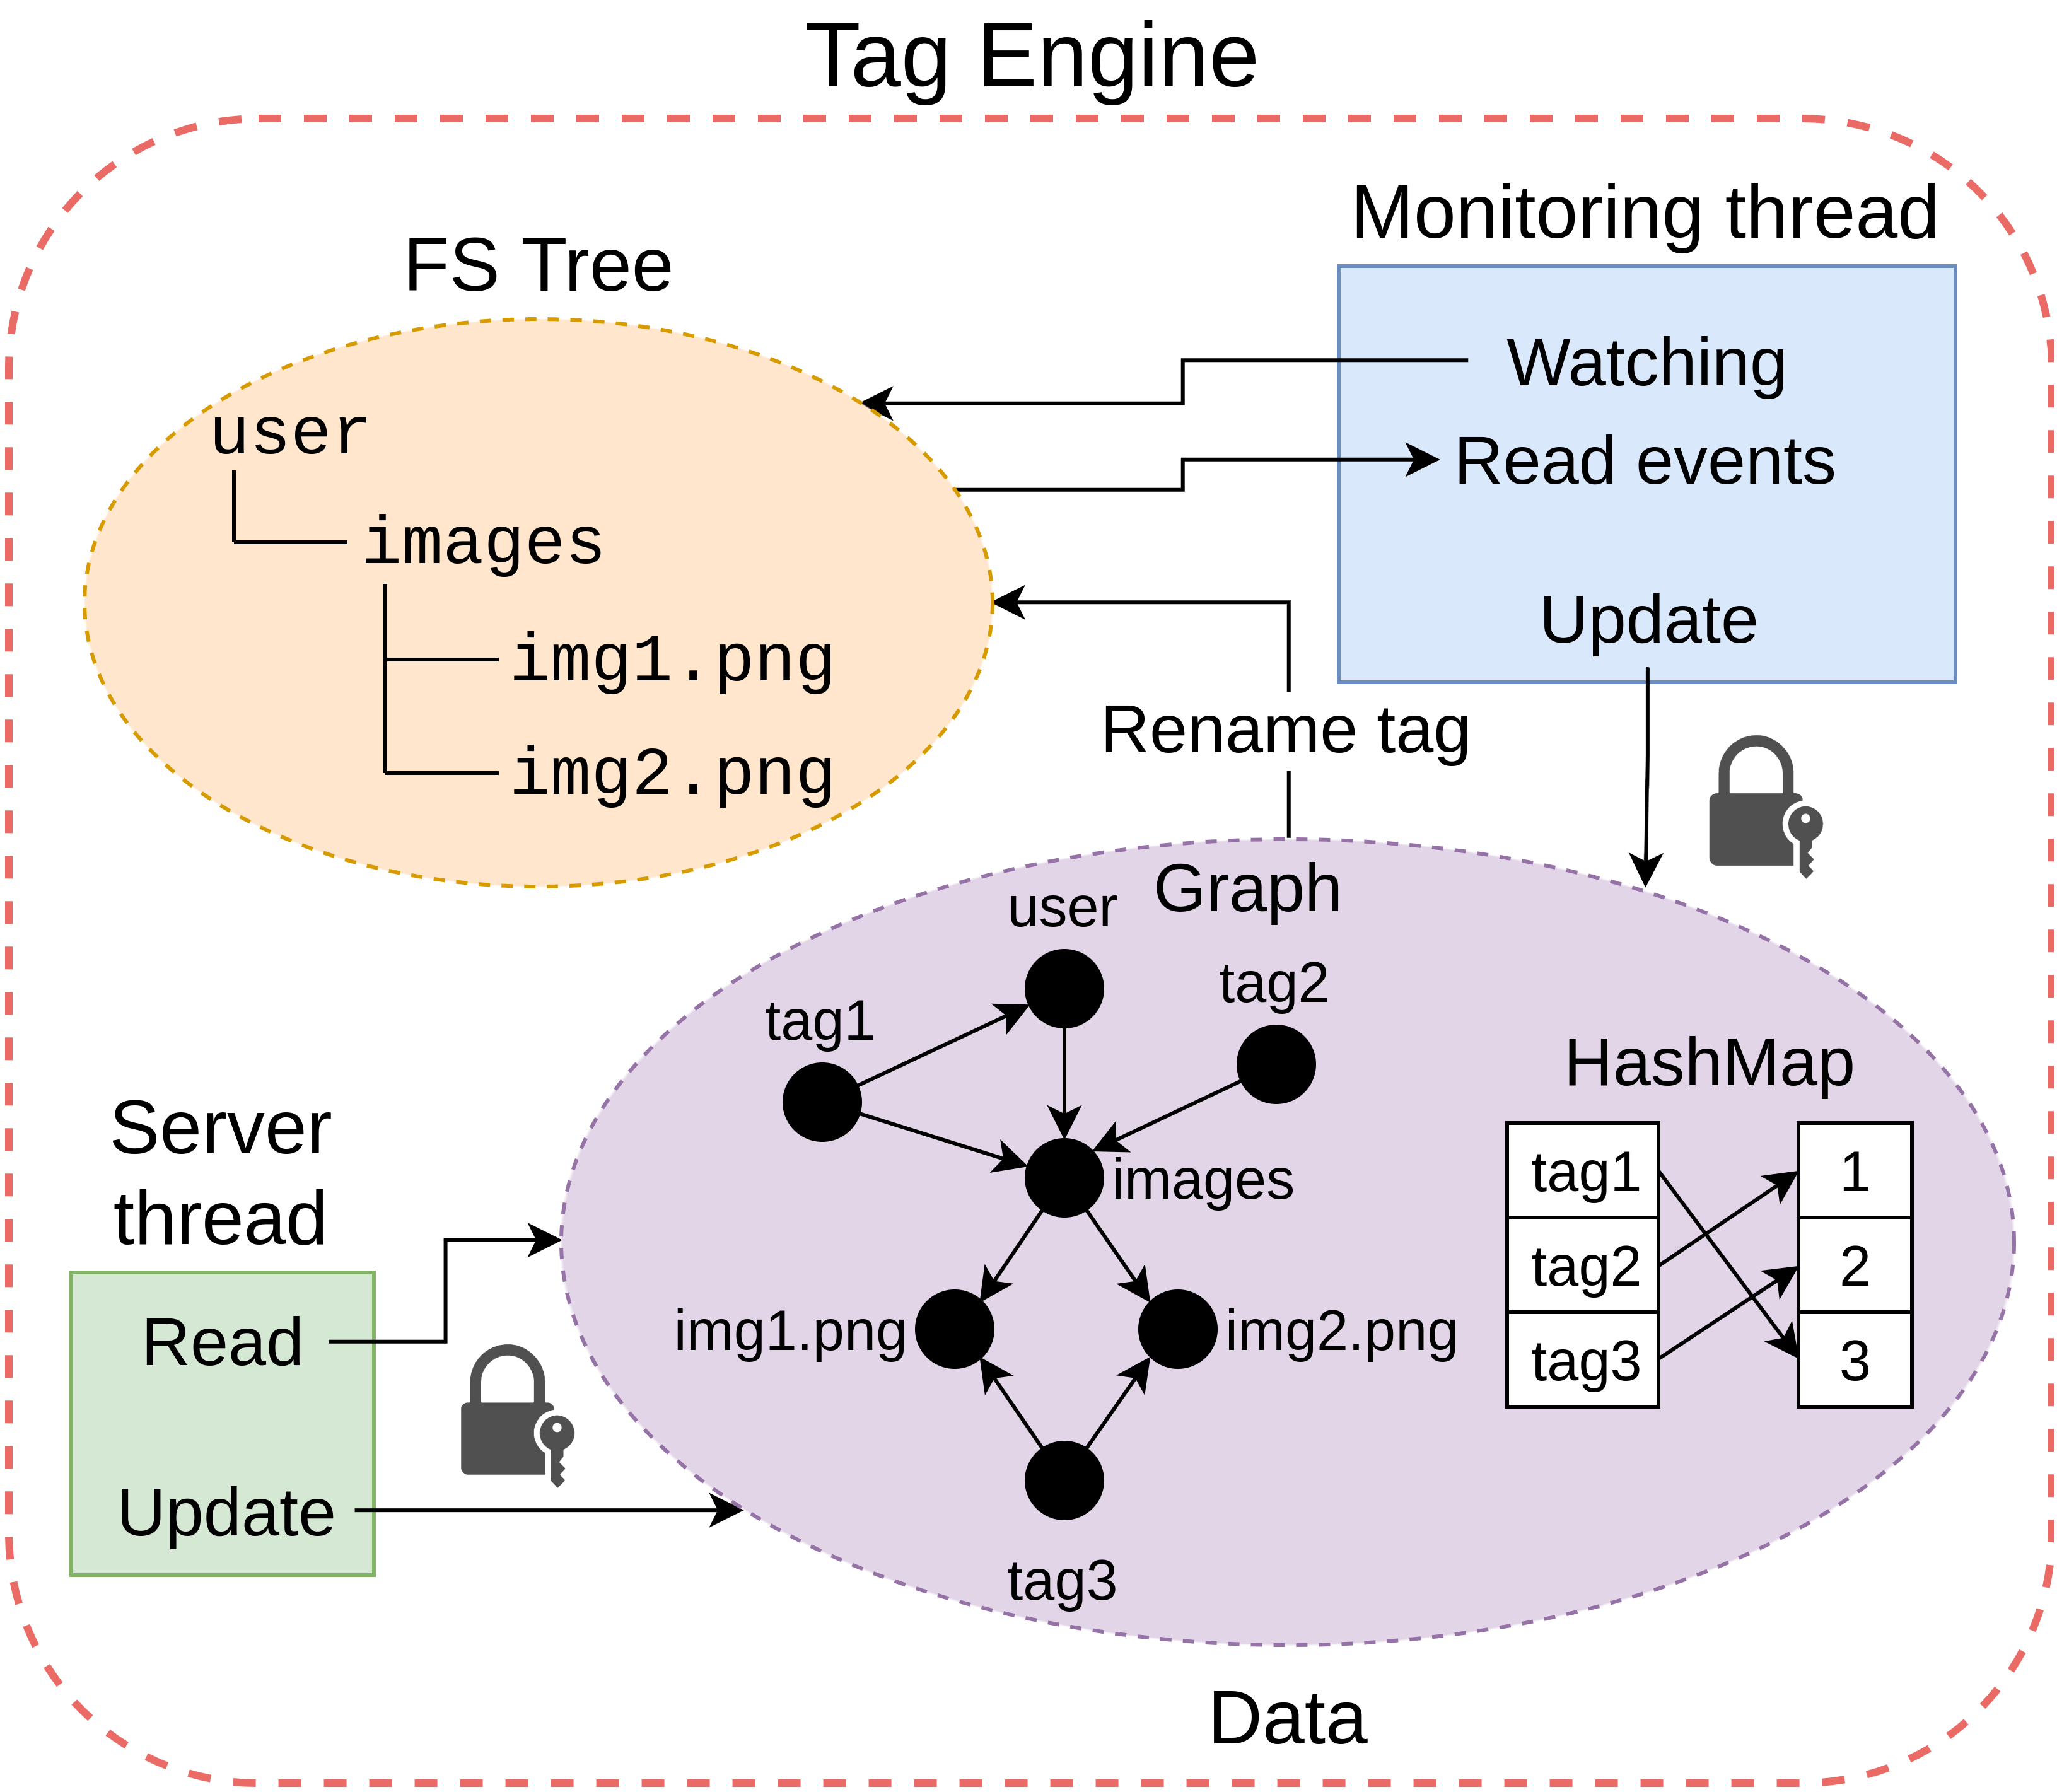
\includegraphics[width=1\textwidth]{images/tag_engine2.png}
                \end{center}
            \end{figure}
        \end{column}
        \pause
        \begin{column}{.4\textwidth}
        \fontsize{8pt}{9}\selectfont
            \begin{itemize}
                \item Programme "serveur".
                \item Surveille l'arborescence des fichiers.
                \item Les changements sur le FS sont répercutés sur le graphe.
                \item Maintient la relation entre tags, fichiers et répertoires (graphe et hashmap).
                \item Écoute sur une socket les requêtes provenant de Tag Manager.
                \item Retourne la liste des fichiers correspondants à une requête logique (opérateurs OR et AND).
            \end{itemize}
        \end{column}
    \end{columns}
\end{frame}

\subsection{TagFS}
\begin{frame}
    \frametitle{\subsecname}
    \begin{figure}
        \begin{center}
            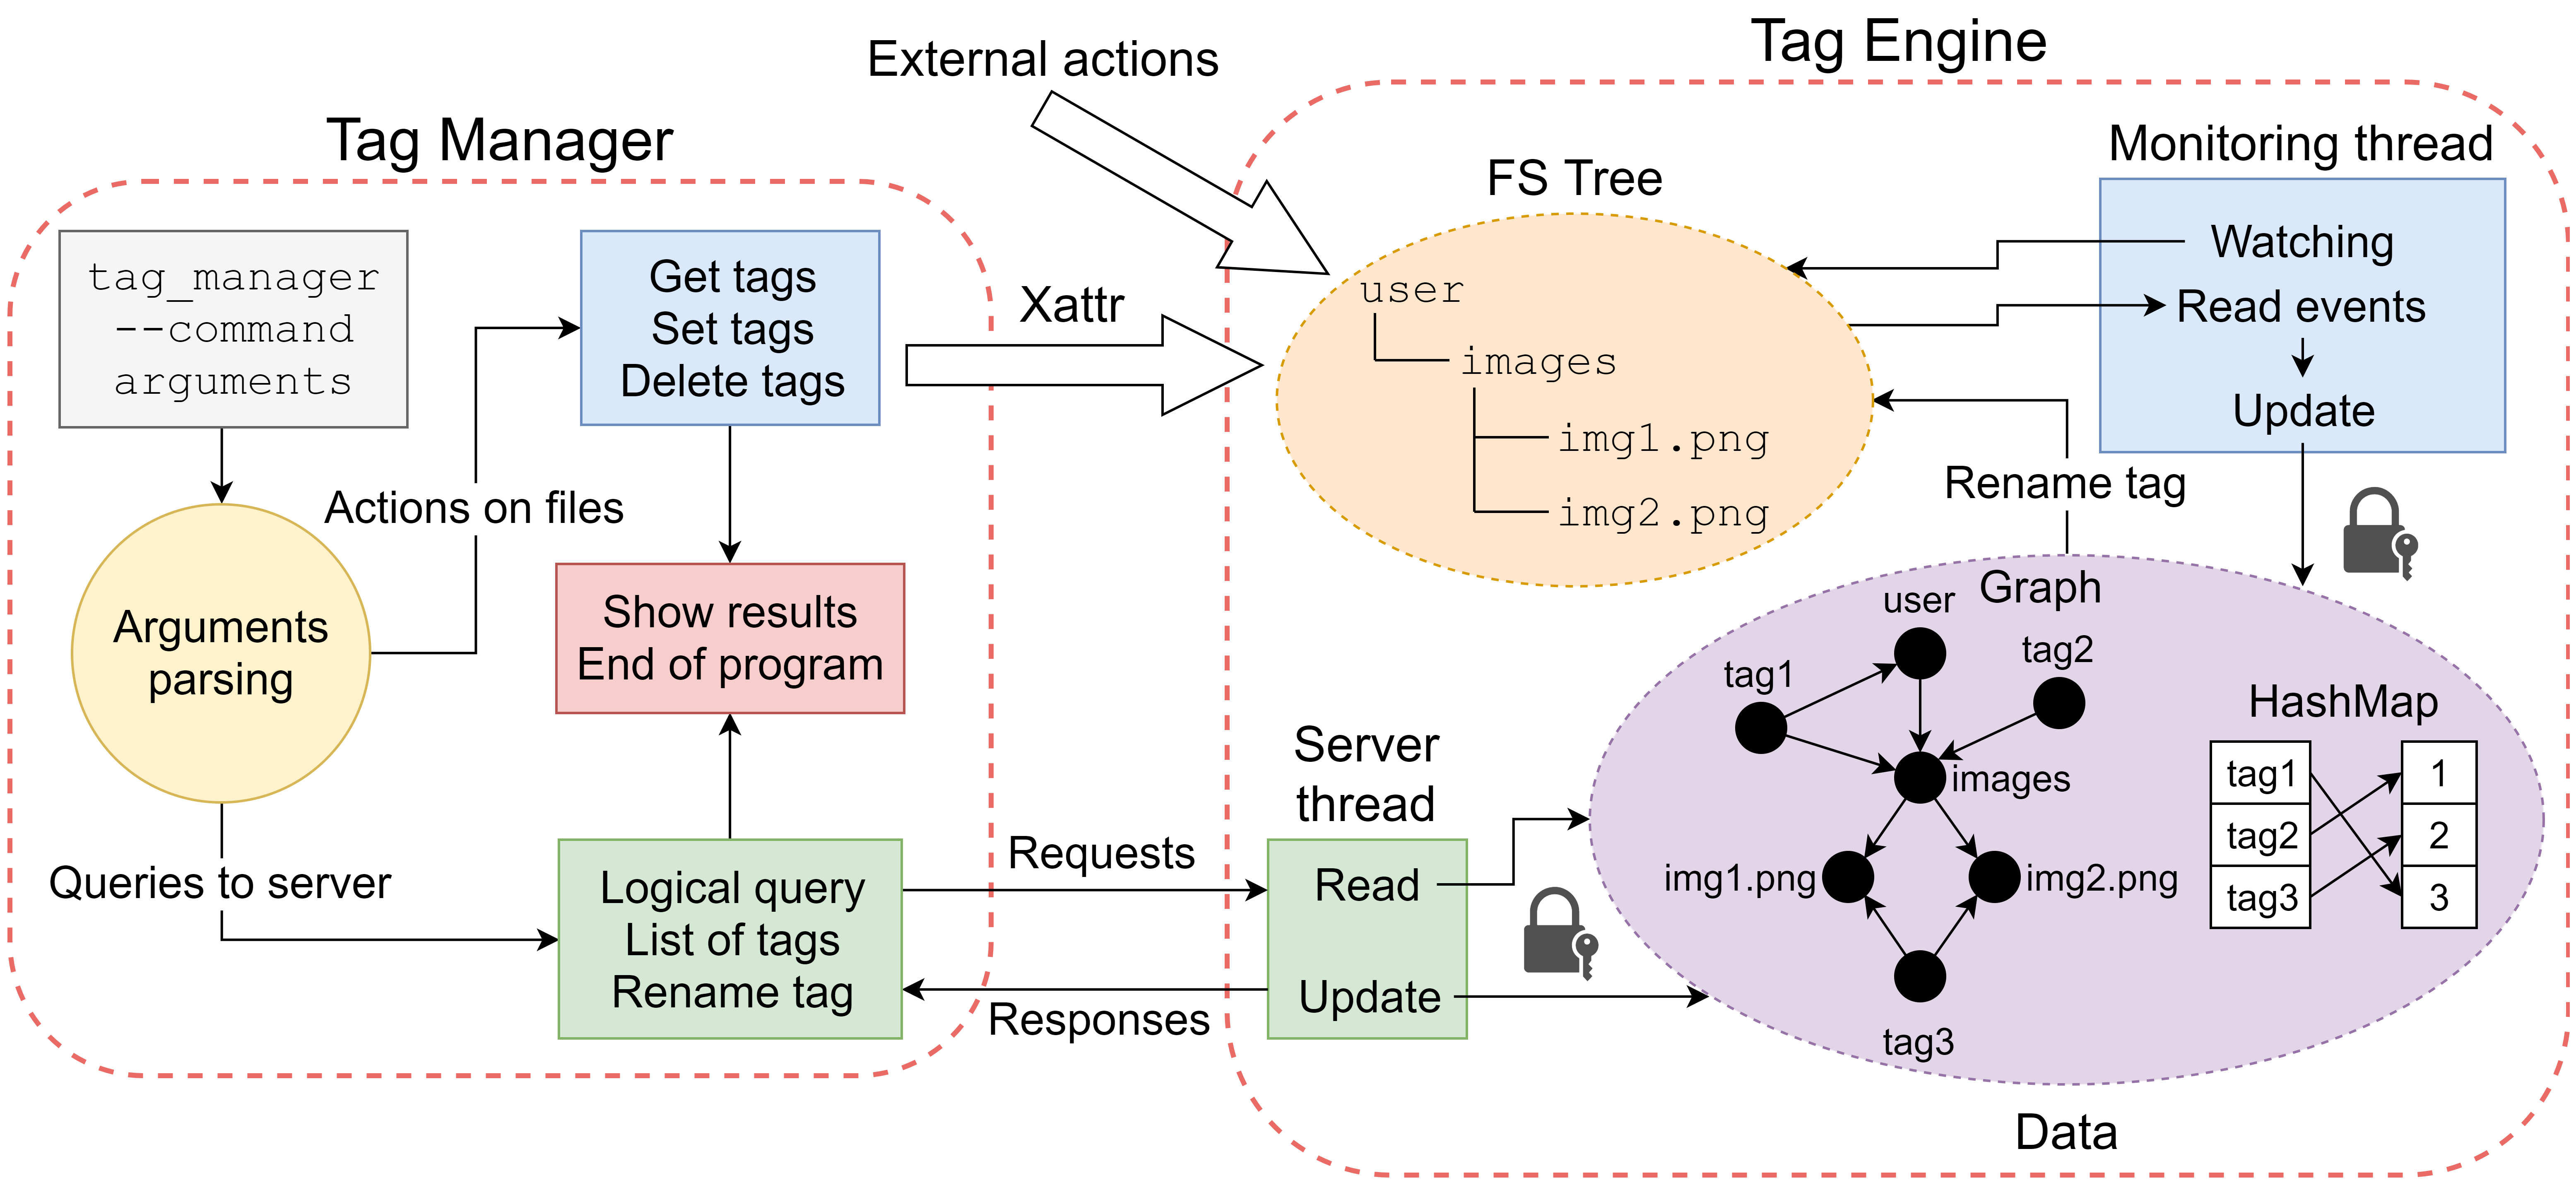
\includegraphics[width=1\textwidth]{images/tagfs4.png}
        \end{center}
    \end{figure}
\end{frame}

\subsection{Démo}
\begin{frame}
    \frametitle{\subsecname}
    \begin{center}
        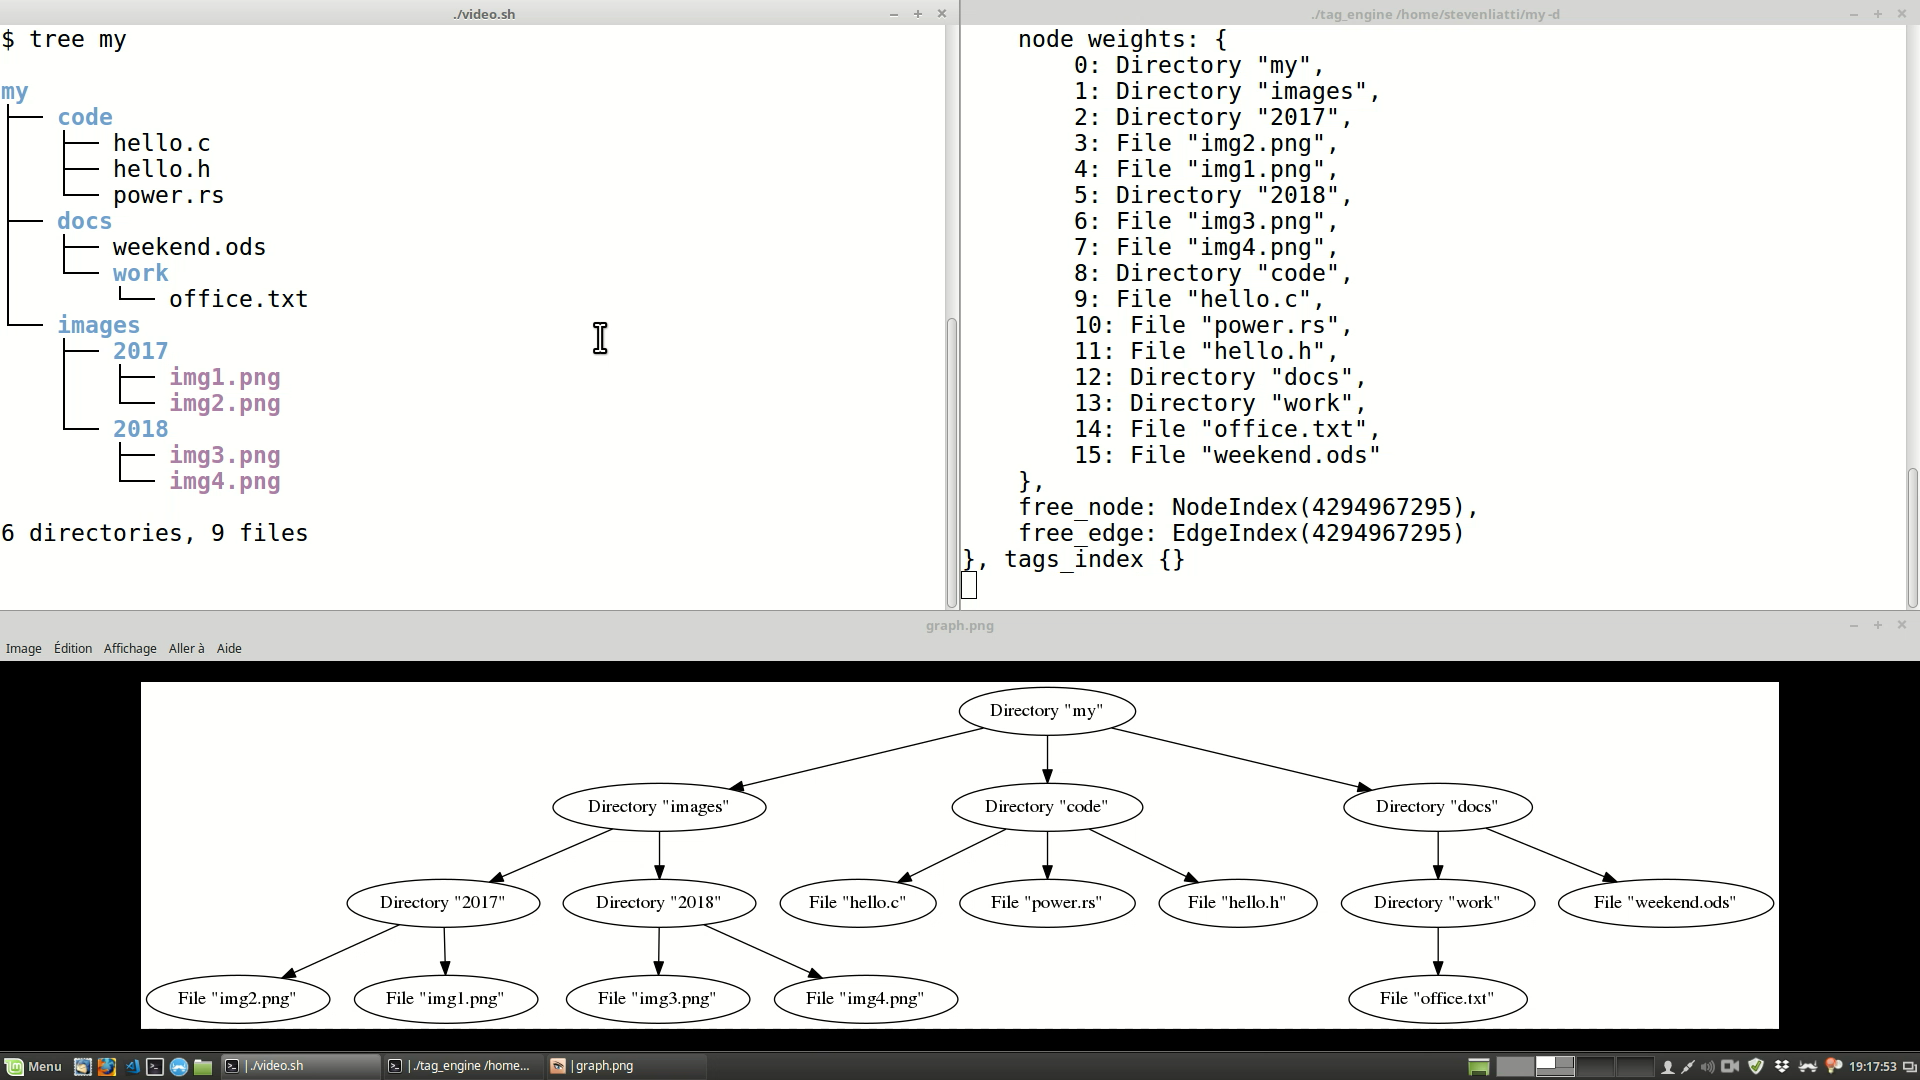
\includegraphics[width=0.8\textwidth]{images/video.png}
        \bigbreak
        \movie[externalviewer]{Vidéo}{video.mp4}
    \end{center}
\end{frame}

%%%%%%%%%%%%%%%%%%%%%%%%%%%%%%%%%%%%%%%%%%%%%%%%%%%%%%%%%%%%%%%%%%%%%%%%%%%%%%%%%%%%%%%%%%%%%%%%%%%
%%%%%%%%%%%%%%%%%%%%%%%%%%%%%%%%%%%%%%%%%%%%%%%%%%%%%%%%%%%%%%%%%%%%%%%%%%%%%%%%%%%%%%%%%%%%%%%%%%%
\section{Discussion}
\subsection{Mesures de performances}
\begin{frame}
    \frametitle{\subsecname}
    \begin{columns}[T]
        \begin{column}{.35\textwidth}
        \fontsize{6pt}{8}\selectfont
            \begin{tabularx}{4cm}{|p{1cm}|p{1cm}|X|} \hline
                \textbf{Répertoire} & \textbf{Sous-répertoires} & \textbf{Fichiers} \\ \hline
                Android & 15'172 & 112'046 \\ \hline
                android-studio & 3'331 & 13'287 \\ \hline
                bin & 553 & 9'306 \\ \hline
                Documents & 15'442 & 64'486 \\ \hline
                Dropbox & 2'377 & 8'659 \\ \hline
                Images & 5 & 863 \\ \hline
                Musique & 135 & 1'352 \\ \hline
            \end{tabularx}
        \end{column}
        \pause
        \begin{column}{.65\textwidth}
            \begin{figure}
                \begin{center}
                    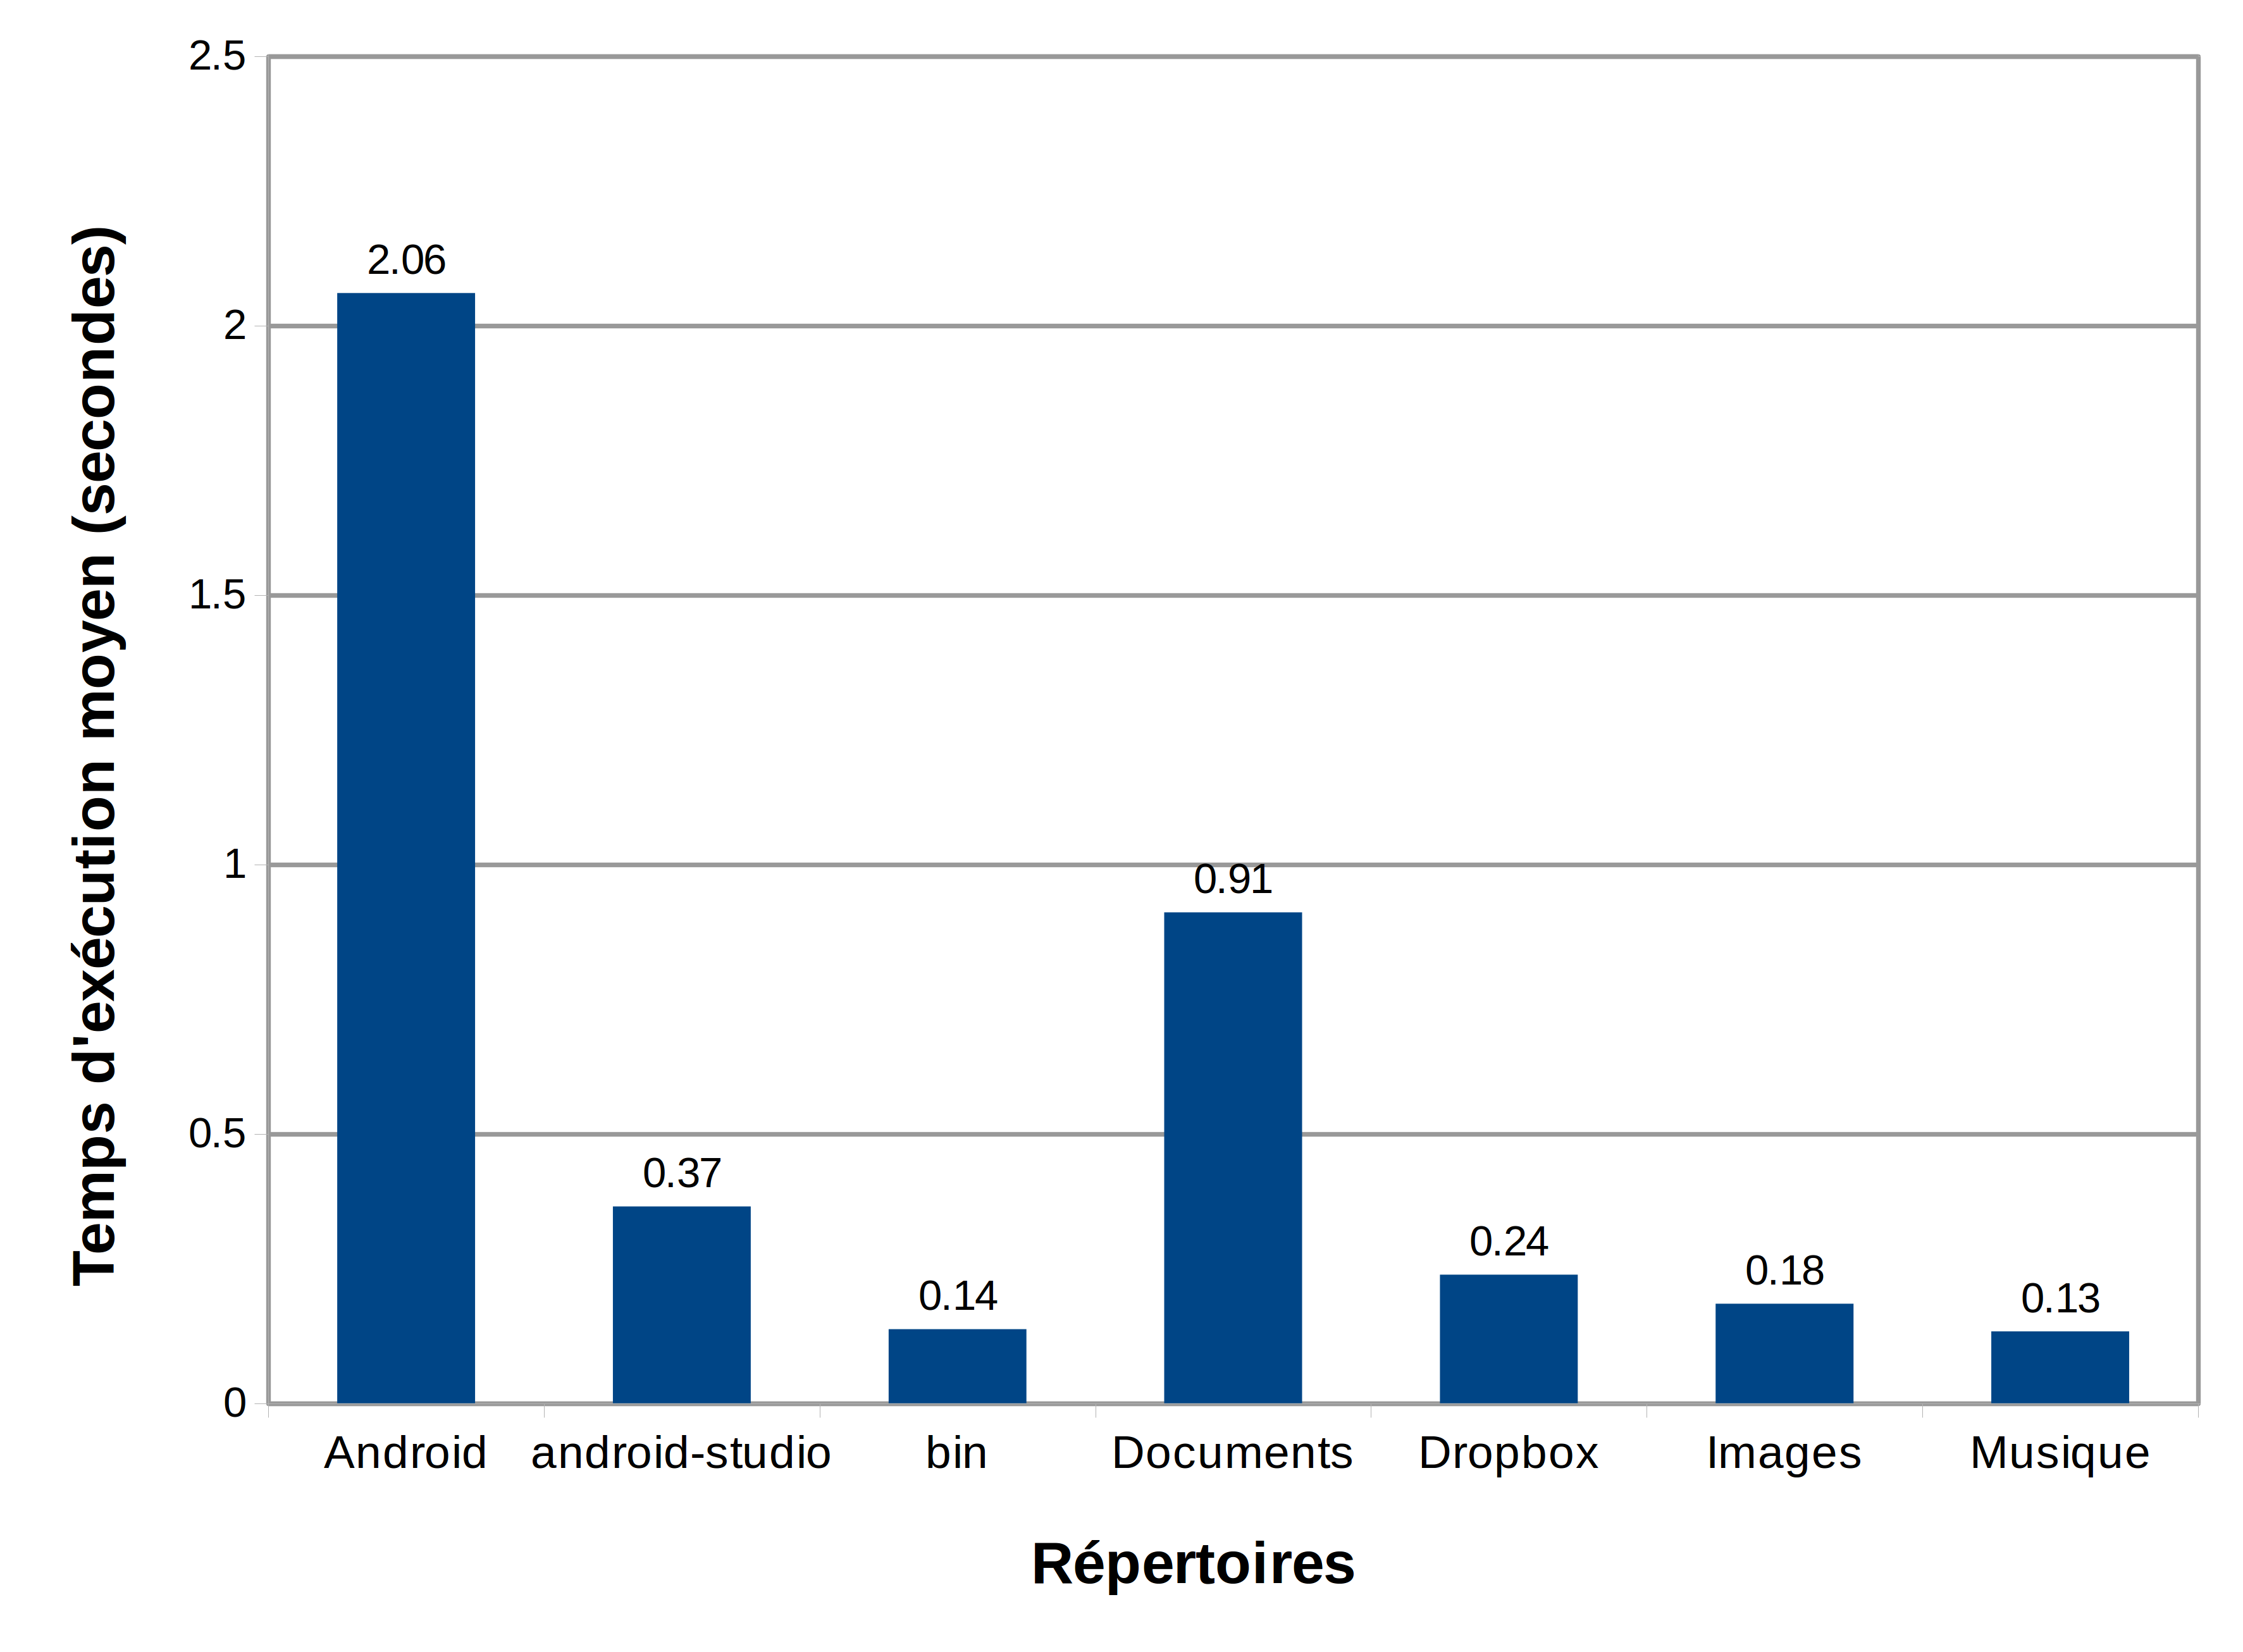
\includegraphics[width=1\textwidth]{images/histo3.png}
                \end{center}
            \end{figure}
        \end{column}
    \end{columns}
\end{frame}

%%%%%%%%%%%%%%%%%%%%%%%%%%%%%%%%%%%%%%%%%%%%%%%%%%%%%%%%%%%%%%%%%%%%%%%%%%%%%%%%%%%%%%%%%%%%%%%%%%%
%%%%%%%%%%%%%%%%%%%%%%%%%%%%%%%%%%%%%%%%%%%%%%%%%%%%%%%%%%%%%%%%%%%%%%%%%%%%%%%%%%%%%%%%%%%%%%%%%%%
\subsection{Améliorations}
\begin{frame}
    \frametitle{\subsecname}
    \begin{itemize}
        \pause
        \item GUI : environnement de bureau ou application web.
        \pause
        \item Daemon pour Tag Engine.
        \pause
        \item Ajout de nouveaux répertoires de surveillance (partiel).
        \pause
        \item Gestion des périphériques amovibles (limitation inotify).
        \pause
        \item Cache des dernières requêtes logiques adressées au serveur.
        \pause
        \item Ajouter des opérateurs logiques (NOT).
    \end{itemize}
\end{frame}

\section{Conclusion}
\subsection{Bilan personnel}
\begin{frame}
    \frametitle{\subsecname}
    \begin{itemize}
        \pause
        \item Conception d'un moteur de gestion de tags.
        \pause
        \item Étude du langage Rust.
        \pause
        \item Diverses technologies et approches.
        \pause
        \item Cahier des charges rempli.
        \pause
        \item Progression personnelle : technologies, bonnes pratiques, démarche.
    \end{itemize}
\end{frame}

%%%%%%%%%%%%%%%%%%%%%%%%%%%%%%%%%%%%%%%%%%%%%%%%%%%%%%%%%%%%%%%%%%%%%%%%%%%%%%%%%%%%%%%%%%%%%%%%%%%
%%%%%%%%%%%%%%%%%%%%%%%%%%%%%%%%%%%%%%%%%%%%%%%%%%%%%%%%%%%%%%%%%%%%%%%%%%%%%%%%%%%%%%%%%%%%%%%%%%%
\subsection{Remerciements}
\begin{frame}
    \frametitle{\subsecname}
    \begin{itemize}
        \item Florent Glück
        \item Orestis Malaspinas
        \item Joël Cavat
    \end{itemize}
\end{frame}

\subsection{Références}
\begin{frame}[allowframebreaks]
    \frametitle{\subsecname}
	\bibliographystyle{unsrt}
	\bibliography{bib}
\end{frame}


\end{document}
